
\chapter{Analise de Resultados} % (fold)
\label{cha:analise_de_resultados}

Neste capitulo serão analisados os resultados obtidos no capitulo anterior, que servirão de motivo para a tomada de decisão de como a contribuição será realizada. Resultados como desempenho, consumo de memória e custos de implementação serão apontadas com o objetivo de comparação entre os algoritmos.


\section{\nmu Algorítimos de \textit{string matching} exatos} % (fold)
\label{sec:algor_timos_de_string_matching_exatos}

Para a busca com algorítimos de \textit{string matching} exatos, foram considerado três métodos distintos:

\begin{description}
	\item[Expressão Regular:] Método atual de como a verificação é realizada atualmente. Foi previamente comentado na sessão de \lnameref{sec:algoritimos_de_textit}.
	\item[Knuth-Morris-Pratt:] Método que faz de uso do conceito de autômatos de estados para agilizar a busca. Previamente apresentado na sessão \ref{ssub:knuth_morris_pratt_}.
	\item[Rabin-Karp:]  Método que faz de uso de \textit{hash}. Foi previamente comentado na sessão \ref{ssub:rabin_karp}.
\end{description}

Após a coleta de $150$ chamadas de cada pacote usando os algorítimos apontados acima, a \autoref{ssub:rabin_karp} foi criada contendo a mediana dos tempos de execução de cada método para os pacotes selecionados.

\begin{figure}[htbp]
  \centering
  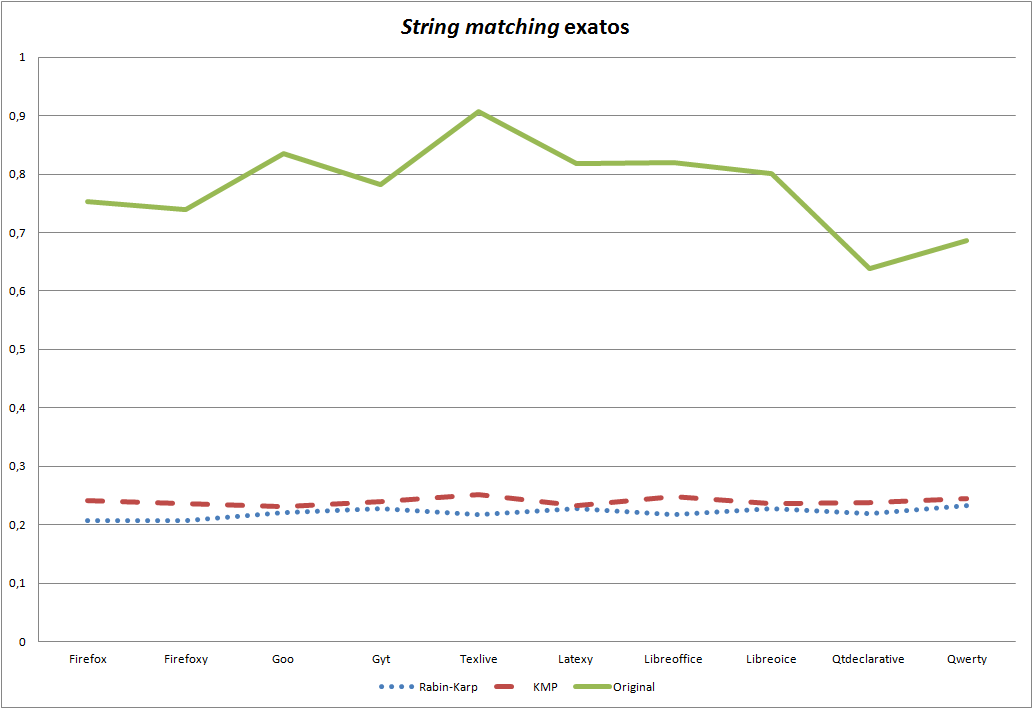
\includegraphics[width=0.95\textwidth]{figuras/tempo-rk_kmp_std}
  \caption{Estimativa de tempo para pacotes usando algorítimos de busca exata}
  \label{tempo_rk_kmp_std}
\end{figure}

Como podemos observar, tanto o \textit{Rabin-Karp} quanto o \textit{KMP} tiveram um rendimento de cerca de $\frac{1}{3}$ do tempo gasto atualmente com o uso de expressões regulares, sendo no tempo geral, o método de \textit{Rabin-Karp} possui um desempenho ligeiramente melhor.


\begin{figure}[htbp]
  \centering
  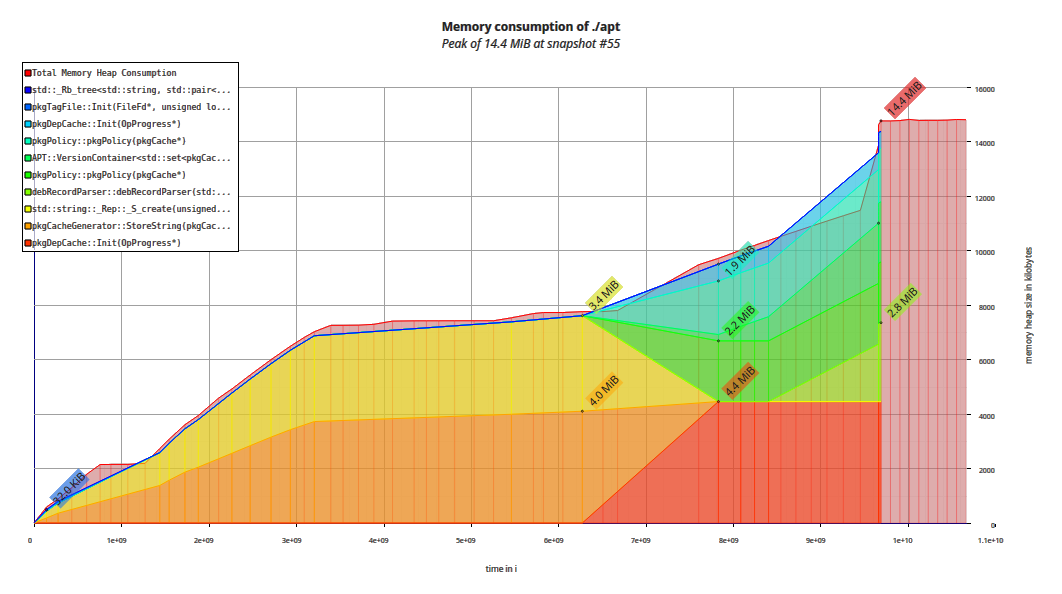
\includegraphics[width=0.95\textwidth]{figuras/memory_rk.png}
  \caption{Apontamento de uso de memória com uso do método de \textit{Rabin-Karp}}
  \label{memory_rk}
\end{figure}

O consumo total de memória para ambos os métodos, \textit{Rabin-Karp} na \autoref{memory_rk} e expressões regulares na \autoref{memory_std},  apresentaram resultados similares, porém o método de \textit{Rabin-Karp} faz um uso de memória mais pontual, alcançando o pico de consumo ao final do processo, quando esta prestes a liberar os recursos. Já o método de expressões regulares apresenta um consumo mais linear de memória. 


\begin{figure}[htbp]
  \centering
  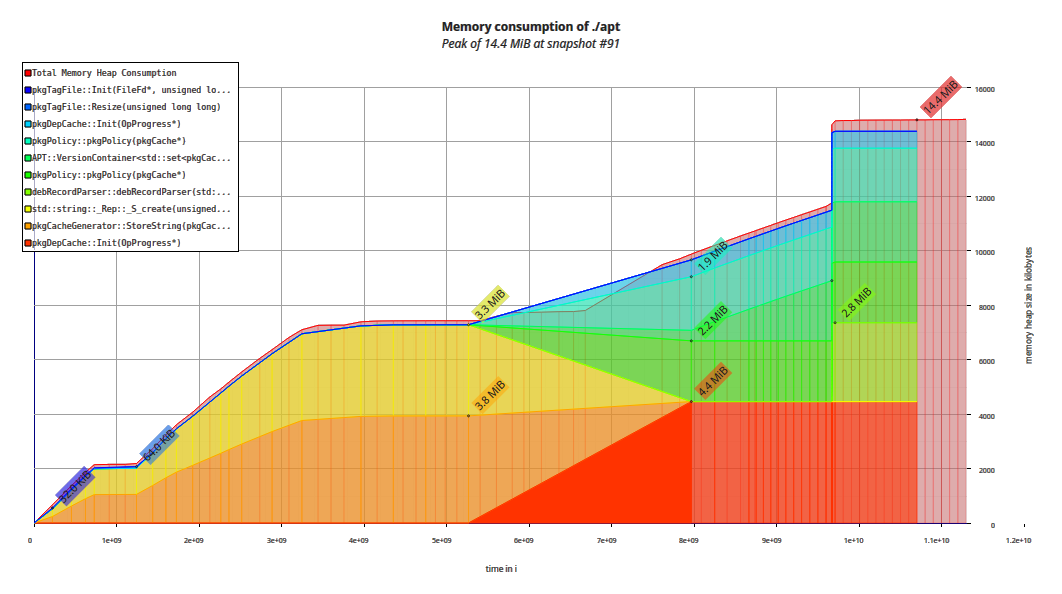
\includegraphics[width=0.95\textwidth]{figuras/memory_regex.png}
  \caption{Apontamento de uso de memória com uso de expressões regulares}
  \label{memory_std}
\end{figure}

Um gasto mais prologado de memória vem a ser prejudicial para sistemas em que diversos processos possam estar sendo executados em conjunto, todavia o grau de consumo é muito baixo para o posicionamento de que o consumo por um período mais extenso venha a ser prejudicial, visto que para um sistema com $2GB$ de memória RAM, $15MB$ seria um valor irrisório de menos de $1\%$ do total de recurso disponível.
% chapter analise_de_resultados (end)


\section{Algoritmos de \textit{string matching} inexatos} % (fold)
\label{sec:algor_timos_de_string_matching_inexatos}

Para a busca com algoritmos de \textit{string matching} inexatos, foram considerado dois métodos distintos:

\begin{description}
	\item[Levenshtein:] Método voltado para correção de erros. Foi previamente comentado na \autoref{sec:leveinstein}.
	\item[Coeficiente de Sørensen–Dice:] Método que faz de uso do conceito de autômatos de estados para agilizar a busca. Previamente apresentado na \autoref{ssub:s_rensen_dice_coefficient}.
\end{description}

Para analise de desempenho, foram coletadas 150 amostras de tempo para 10 buscas por pacotes distintos das quais metade eram de pacotes que não existiam, semelhante realizado para os \lnameref{sec:algor_timos_de_string_matching_exatos}. A \autoref{tempo_rk_kmp_std_lev_dic} retrata a mediana destes tempos.

\begin{figure}[htbp]
  \centering
  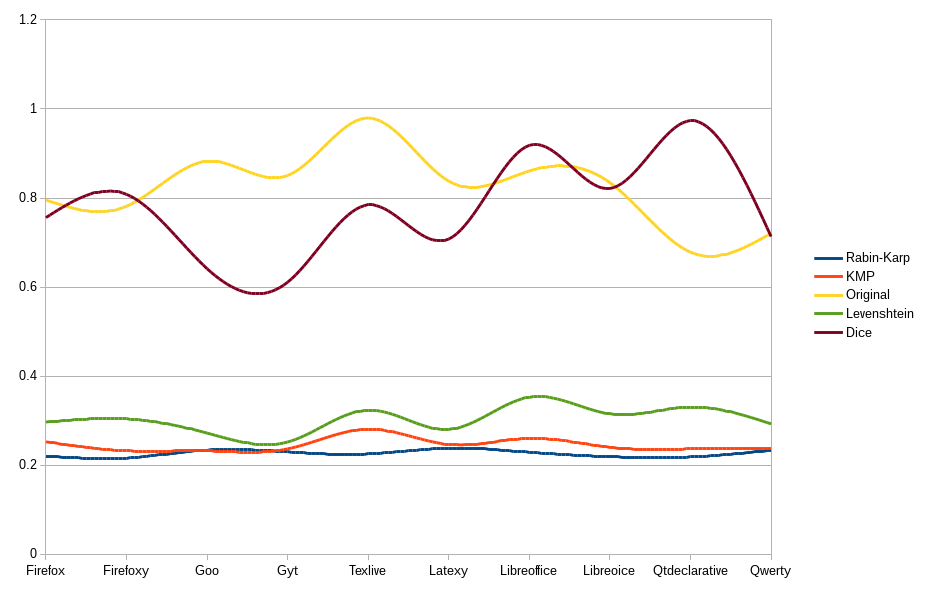
\includegraphics[width=0.95\textwidth]{figuras/tempo-rk_kmp_std_lev_dice}
  \caption{Estimativa de tempo para pacotes usando algoritmos de busca inexata}
  \label{tempo_rk_kmp_std_lev_dic}
\end{figure}

Como apresentado na primeira etapa deste trabalho\footnote{Trabalho de conclusão de curso 1: Algoritmo para Qualificação das Saídas de Buscas em
Gerenciadores de Repositórios de Distribuições Linux}, o algoritmo de \textit{Leveinstein} apresenta um dos melhores tempos para buscas inexatas de \textit{strings}. A \autoref{tempo_rk_kmp_std_lev_dic} reforça essa afirmação, ao mostrar que o tempo de resposta deste algoritmo é inferior ao tempo gasto para buscas com expressões regulares e ficando pouco acima do tempo necessário para realizar buscas exatas com o algoritmo de  \textit{Rabin-Karp}.

% \section{Resultados Gerais} % (fold)
% \label{sec:resultados_gerais}

% subsection tempo (end)
% section resultados_gerais (end)
\chapter{Conclusão} % (fold)
\label{cha:dificuldades_encontradas}


O uso de algoritmos para substituir o uso de expressões regulares apresentam ganhos de desempenho notáveis, oferecendo buscas que fazem menos uso de recursos e apresentam os resultados em menor tempo, porém a economia de memoria não se mostrou  

% \section*{Guia de estilo} % (fold)
% \label{sec:guia_de_estilo}

O grupo responsável pela manutenção e evolução do {\code APT} segue um guia de estilo de código extremamente peculiar, apresentado no \autoref{styleguide}. De acordo com o guia de estilo seguido, as edentações devem ser realizadas com espaço de três para cada nível, porém a cada oito espaços, devem ser substituídos por tabulações.

% \section*{Testes quebrados} % (fold)
% \label{sec:testes_de_concorr_ncias}

Um hábito comum com o desenvolvimento da aplicação é o fato de manter \textit{builds} em que o \textit{status} na aplicação \textit{Travis CI} quebrando, devido ao fato de grande parte dos testes serem realizados com chamadas de concorrências. Devido ao tempo e ordem destas chamadas não serem deterministas, muitas vezes um teste falha por estar definido uma ordem diferente do resultado obtido pela chamada em concorrência.
Este mal habito é um dos motivos de múltiplas contribuições serem recusadas, visto que o GitHub aponta a \textit{build} como quebrada e não recomenda aceitar. Outra falha comum nos testes é um cenário para adquirir o mesmo arquivo múltiplas vezes. Este teste infelizmente falha devido a instabilidade da plataforma de integração continua (\textit{Travis CI}) que muitas das vezes resulta em um \textit{timeout} no \textit{download} do arquivo, gerando a falha no teste.


% \section*{Coesão e Coerência} % (fold)
% \label{sec:coes_o_e_coer_ncia}

Para um software de grande responsabilidade como o APT, esperava-se classes pequenas com métodos objetivos e coesos, porém é comum observar métodos e funções com mais de trinta linhas com múltiplas obrigações. Como consequência, há funções com mesmos objetivos ou semelhantes, provavelmente devido a dificuldade em se encontrar um método dedicado para uma única tarefa.

% chapter dificuldades_encontradas (end)
